\chapter{Revisión Bibliográfica}
\label{ch:litRev}

% Estado del arte general y específico del tema investigado.
% Incluir referencias de los últimos 5 años. Máximo 15 páginas.

\section{Programación semidefinida}
\label{sec:programacion_semidefinida}

La \acrfull{sdp} es una clase de optimización convexa en la que se optimiza una función
lineal sujeta a restricciones lineales y a una restricción de semidefinitud positiva sobre
una matriz simétrica. En términos generales, extiende la programación lineal al reemplazar
la condición de no negatividad de un vector por la pertenencia de una matriz al cono de
matrices semidefinidas positivas. Esta generalización permite modelar problemas donde la
variable de decisión no es solo un vector, sino una matriz cuyas propiedades espectrales
deben cumplir ciertas condiciones.

Sea $\mathbb{S}^n$ el espacio de matrices simétricas reales de orden $n$. Una matriz
$X\in\mathbb{S}^n$ es semidefinida positiva si
\[
    z^\top X z \geq 0, \qquad \forall z\in\mathbb{R}^n,
\]
lo que se denota por $X\succeq 0$. El conjunto
\[
    \mathbb{S}_+^n=\{X\in\mathbb{S}^n: X\succeq 0\}
\]
forma un cono convexo. Esta convexidad es central: aunque la restricción $X\succeq 0$ es
no lineal en el sentido de que impone condiciones sobre los autovalores de $X$, el conjunto
factible resultante sigue siendo convexo.

Una forma estándar primal de un problema de programación semidefinida es
\[
\begin{aligned}
    \min_{X\in\mathbb{S}^n}\quad & \langle C,X\rangle \\
    \text{sujeto a}\quad & \langle A_i,X\rangle = b_i,
        \qquad i=1,\ldots,m,\\
    & X\succeq 0,
\end{aligned}
\]
donde $C,A_1,\ldots,A_m\in\mathbb{S}^n$, $b\in\mathbb{R}^m$ y
$\langle A,X\rangle=\mathrm{tr}(AX)$ corresponde al producto interno de Frobenius para
matrices simétricas. En esta formulación, la función objetivo y las restricciones de igualdad
son lineales en la variable matricial $X$, mientras que la restricción cónica $X\succeq 0$
garantiza que la solución pertenezca al cono semidefinido positivo.

El problema dual asociado puede escribirse como
\[
\begin{aligned}
    \max_{y\in\mathbb{R}^m}\quad & b^\top y \\
    \text{sujeto a}\quad & C-\sum_{i=1}^{m} y_i A_i \succeq 0.
\end{aligned}
\]
La restricción dual exige que una combinación afín de matrices simétricas sea semidefinida
positiva. Esta condición se conoce como una desigualdad matricial lineal o \textit{linear
matrix inequality} (LMI). Por ello, muchos problemas formulados mediante LMIs pueden verse
directamente como programas semidefinidos.

La programación semidefinida incluye como casos particulares a la programación lineal y a
ciertas formas de programación cuadrática convexa. En programación lineal, la restricción
de no negatividad $x\geq 0$ puede interpretarse como la pertenencia de una matriz diagonal
$\mathrm{diag}(x)$ al cono $\mathbb{S}_+^n$. En \acrshort{sdp}, esta idea se amplía al permitir
matrices completas o por bloques, lo que hace posible capturar interacciones entre variables
mediante términos fuera de la diagonal. Esta capacidad explica su relevancia en áreas como
control robusto, optimización combinatoria, diseño estructural y relajaciones convexas de
problemas no convexos.

Según la descripción clásica de Vandenberghe y Boyd, un programa semidefinido minimiza una
función lineal bajo la condición de que una combinación afín de matrices simétricas sea
semidefinida positiva; aunque esta restricción es no lineal y no suave, preserva la
convexidad del problema~\cite{vandenbergheSemidefiniteProgramming1996}. Esta combinación de
expresividad y estructura convexa ha permitido extender a \acrshort{sdp} muchas ideas
algorítmicas desarrolladas originalmente para programación lineal, en particular los métodos
de punto interior primal-dual.

\subsection{Solvers para programación semidefinida}
\label{sec:solvers_sdp}

El desarrollo de solvers para \acrshort{sdp} está estrechamente ligado a la estructura cónica del
problema. Aunque la formulación es convexa, resolver instancias grandes puede ser costoso por
la presencia de variables matriciales, restricciones de semidefinitud y sistemas lineales densos o
mal condicionados. Por ello, la literatura y el software especializado han explorado distintas
familias algorítmicas, cada una con ventajas y limitaciones según el tamaño, la densidad y la
estructura de la instancia.

\subsubsection{Familias algorítmicas}
\label{subsec:familias_algoritmicas_sdp}

La familia más clásica corresponde a los métodos de punto interior primal-dual. Estos métodos
generalizan ideas de programación lineal al cono semidefinido positivo y construyen una secuencia
de iterados que se aproximan simultáneamente a la factibilidad primal, factibilidad dual y
optimalidad. Su fortaleza principal es la robustez numérica y la buena precisión en instancias
pequeñas y medianas. Sin embargo, cada iteración suele requerir la formación y resolución de un
sistema de Schur asociado a las restricciones, cuyo costo puede crecer rápidamente con el número
de restricciones y el tamaño de los bloques semidefinidos.

Una segunda familia corresponde a los métodos de escalamiento dual. Estos métodos trabajan
principalmente desde el problema dual y buscan reducir los requerimientos de memoria frente a
ciertas variantes primal-dual completas. En lugar de construir iterados primal y dual con el mismo
nivel de detalle, explotan la estructura dual para obtener pasos más económicos en problemas
donde el sistema asociado sería demasiado costoso.

Una tercera línea corresponde a los métodos de Lagrangiano aumentado y Newton-CG. Estos
métodos son especialmente relevantes para instancias de mayor escala, donde formar y factorizar
sistemas densos puede ser prohibitivo. Su idea general es resolver una secuencia de subproblemas
regularizados, usando pasos de Newton aproximados o métodos iterativos. En comparación con
los métodos de punto interior, suelen sacrificar parte de la precisión de alta tolerancia a cambio
de una mejor escalabilidad en problemas grandes.

La coexistencia de estas familias muestra que no existe un solver universalmente dominante. Un
método puede ser competitivo en instancias pequeñas y densas, mientras otro puede destacar en
problemas dispersos, con muchas restricciones o con bloques grandes. Esta variabilidad motiva el
análisis del desempeño de los solvers en función de las características de cada
instancia.

\subsubsection{SDPT3}
\label{subsec:solver_sdpt3}

SDPT3 fue desarrollado por Kim-Chuan Toh, Michael J. Todd y Reha H. Tütüncü. Es uno de los
solvers más usados dentro de la familia de métodos de punto interior primal-dual y está
implementado en MATLAB. Resuelve problemas semidefinidos, cuadráticos y lineales cónicos. Su
versión 4.0 incorpora direcciones predictor-corrector y variantes HKM/NT, por lo que se ha
convertido en una referencia habitual para experimentos comparativos en \acrshort{sdp}
\cite{tohImplementationUsageSDPT32012a}.

\subsubsection{SeDuMi}
\label{subsec:solver_sedumi}

SeDuMi fue desarrollado originalmente por Jos F. Sturm. También pertenece a la familia de
métodos de punto interior primal-dual, pero fue diseñado como un solver más general para
optimización sobre conos simétricos. Además de programación semidefinida, soporta conos de
segundo orden y programación lineal. Su uso se popularizó por la integración con MATLAB y por
su capacidad de resolver formulaciones cónicas expresadas desde lenguajes de modelamiento. En
comparación con SDPT3, comparte el enfoque primal-dual, pero difiere en la implementación de
las direcciones de búsqueda y en el tratamiento numérico del sistema cónico
\cite{sturmUSINGSEDUMI1022001}.

\subsubsection{SDPA}
\label{subsec:solver_sdpa}

SDPA fue desarrollado por el grupo del proyecto SDPA, asociado a Makoto Yamashita, Katsuki
Fujisawa, Masakazu Kojima y colaboradores. Es un solver especializado para programación
semidefinida desarrollado en C++. También se basa en métodos de punto interior primal-dual,
pero se distingue por estar estrechamente asociado al formato SDPA y por ofrecer ejecutables
independientes del entorno MATLAB. Esta característica lo vuelve útil en pipelines experimentales
automatizados, donde se requiere ejecutar muchas instancias desde archivos de entrada
estandarizados \cite{SDPAOfficialPage}.

\subsubsection{CSDP}
\label{subsec:solver_csdp}

CSDP fue desarrollado por Brian Borchers. Es una biblioteca escrita en C para resolver programas
semidefinidos mediante métodos de punto interior. Su diseño enfatiza portabilidad y uso como
biblioteca o ejecutable externo, lo que permite integrarlo en flujos de benchmarking sin depender
de entornos interactivos. En estudios comparativos, CSDP suele servir como una línea base
robusta para evaluar comportamiento de solvers de propósito general en \acrshort{sdp}
\cite{borchersCSDPLibrarySemide}.

\subsubsection{DSDP}
\label{subsec:solver_dsdp}

DSDP fue desarrollado por Steven J. Benson, con contribuciones asociadas a Yinyu Ye y Xiong
Zhang en la literatura del solver. Es un ejemplo representativo de los métodos de escalamiento
dual: fue diseñado para resolver problemas semidefinidos y desigualdades matriciales lineales
usando una estrategia de escalamiento dual, con énfasis en eficiencia y bajo consumo de memoria
\cite{bensonDSDP5SoftwareSemidefinite,bensonDSDP5UserGuide2006a}.

\subsubsection{SDPNAL+}
\label{subsec:solver_sdpnal}

SDPNAL+ fue desarrollado por Liuqin Yang, Defeng Sun y Kim-Chuan Toh como una evolución de
la línea SDPNAL. Representa la familia de métodos de Lagrangiano aumentado y Newton-CG:
combina una formulación de Lagrangiano aumentado con pasos de Newton-CG para resolver
subproblemas de gran tamaño. Estas estrategias buscan evitar algunos de los cuellos de botella
de los métodos de punto interior, en particular la necesidad de factorizar sistemas densos de
gran tamaño. A cambio, pueden entregar soluciones con tolerancias más moderadas o requerir
criterios de parada distintos.

Esta diversidad algorítmica justifica analizar el desempeño de los solvers no solo mediante
promedios agregados, sino en función de las propiedades de las instancias. Características como
el número de restricciones, el tamaño de los bloques, la densidad de las matrices, la estructura
del sistema de Schur y el grado de dispersión pueden afectar directamente el costo de las
operaciones dominantes de cada método. Por ello, la comparación empírica de solvers
\acrshort{sdp} requiere considerar tanto el rendimiento observado como la estructura de las
instancias sobre las que dicho rendimiento se mide.
\cite{sunSDPNALMatlabSoftware2019}

\subsection{Librerías de instancias}
\label{subsec:librerias_instancias_sdp}

\paragraph{SDPLIB.}
\label{subsec:benchmark_sdplib}

SDPLIB es una de las bibliotecas clásicas para la evaluación de solvers de programación
semidefinida. Fue propuesta por Brian Borchers con el objetivo de reunir problemas de prueba en
un formato estándar y estimular el desarrollo de software especializado para \acrshort{sdp}. La
versión 1.2 contiene 92 problemas provenientes de distintas aplicaciones, incluyendo diseño de
estructuras tipo \textit{truss}, ingeniería de control y relajaciones semidefinidas de problemas de
optimización combinatoria. Por su diversidad y por el uso de una representación estandarizada,
SDPLIB se convirtió en una referencia habitual para comparar solvers y verificar implementaciones
en instancias de tamaño pequeño y mediano \cite{borchersSDPLIB12Library1999}.

\newpage
\subsection{Benchmarks para programación semidefinida}
\label{sec:benchmarks_sdp}

\paragraph{Benchmarks de Hans Mittelmann.}
\label{subsec:benchmark_mittelmann}

Hans D. Mittelmann es un investigador asociado a Arizona State University, conocido por mantener
benchmarks computacionales de software de optimización numérica. En el contexto de
\acrshort{sdp}, su página \textit{Several SDP-codes on sparse and other SDP problems (also on
GPUs)} reúne comparaciones de distintos códigos SDP sobre problemas dispersos y otros problemas
semidefinidos, incluyendo resultados para solvers clásicos y códigos ejecutados en GPU. Esta
colección complementa la cobertura de SDPLIB con instancias de distintas escalas y procedencias,
y es útil para estudiar el comportamiento de solvers en problemas exigentes, especialmente
cuando las dimensiones o la dispersión de las matrices estresan memoria, tiempo de cómputo o
estabilidad numérica \cite{PlatoasueduFtpSparse_sdphtml}.

\paragraph{DIMACS Library.}
\label{subsec:benchmark_dimacs}

DIMACS corresponde al \textit{Center for Discrete Mathematics and Theoretical Computer
Science}, una iniciativa asociada a Rutgers University orientada a investigación en matemática
discreta, computación teórica y sus aplicaciones. Además de su actividad académica, DIMACS ha
organizado desafíos de implementación cuyo objetivo es comparar algoritmos y software sobre
problemas computacionales bien definidos. En este marco, el \textit{Seventh DIMACS
Implementation Challenge} estuvo dedicado a problemas semidefinidos y problemas de
optimización relacionados.

La biblioteca asociada a este desafío reúne instancias de programas semidefinidos,
cuadráticos y lineales mixtos. Su interés para este trabajo radica en que aporta problemas
originados en formulaciones más generales que incluyen componentes semidefinidas, lo que amplía
la variedad estructural de los benchmarks disponibles. A diferencia de una colección centrada en
un único tipo de aplicación, DIMACS incorpora instancias pensadas para evaluar implementaciones
algorítmicas en un contexto comparativo, por lo que resulta útil para estudiar cómo cambian el
desempeño y la robustez de los solvers frente a estructuras híbridas y restricciones de distinta
naturaleza \cite{DIMACSLibraryMixeda}.

\paragraph{Biq Mac Library.}
\label{subsec:benchmark_biqmac}

Biq Mac Library es una colección de instancias para problemas de corte máximo
(\textit{Max-Cut}) y programación cuadrática binaria 0-1. La biblioteca está asociada al
desarrollo de Biq Mac, un algoritmo \textit{Branch and Bound} que utiliza cotas superiores
obtenidas mediante relajaciones semidefinidas para resolver instancias de tamaño medio de estos
problemas. Por esta razón, aunque las formulaciones originales son combinatoriales, la colección
resulta relevante para evaluar métodos y representaciones basadas en \acrshort{sdp}. Sus
instancias aportan una familia distinta a las colecciones orientadas a control o diseño
estructural, y ayudan a poblar regiones del espacio de instancias con patrones de densidad,
estructura de grafo y bloqueo diferentes \cite{BiqMacLibrarya}.

La fragmentación de estas fuentes tiene consecuencias metodológicas. Si una evaluación usa
instancias provenientes de una sola biblioteca, puede obtener conclusiones sesgadas hacia las
estructuras predominantes en esa colección. Por ejemplo, una biblioteca centrada en problemas
combinatoriales densos puede favorecer o perjudicar familias de solvers distintas a una biblioteca
compuesta por problemas de control dispersos. Por ello, al estudiar algoritmos \acrshort{sdp}, la
diversidad de instancias no es un detalle experimental secundario, sino una condición necesaria
para extraer conclusiones robustas sobre fortalezas y debilidades algorítmicas.

\subsection{Representación de instancias}
\label{sec:representacion_instancias}

\subsubsection{Formato SDPA}
\label{subsec:formato_sdpa}

El formato SDPA denso, usualmente almacenado con extensión \texttt{.dat}, escribe explícitamente
el número de variables, el número de bloques, la estructura de bloques, el vector de costos y las
matrices $F_i$. En esta representación, cada matriz se entrega como un bloque completo, por lo
que resulta directa de leer y útil para ejemplos pequeños. Sin embargo, cuando las matrices tienen
muchos ceros, la representación densa puede crecer innecesariamente y repetir información que no
aporta a la instancia \cite{SDPAFormat}.

El siguiente ejemplo, tomado de la documentación de SDPA para Python, muestra una instancia
con $m=3$ variables, un único bloque de tamaño $2$ y el vector de costos
$c=(48,-8,20)$:

\begin{table}[H]
\centering
\caption{Representación densa del ejemplo en formato SDPA.}
\label{tab:sdpa_format_example}
\begin{minipage}{0.72\textwidth}
\begin{verbatim}
"Example 1: mDim = 3, nBLOCK = 1, {2}"
   3  =  mDIM
   1  =  nBLOCK
   2  =  bLOCKsTRUCT
{48, -8, 20}
{ {-11,  0}, { 0, 23} }
{ { 10,  4}, { 4,  0} }
{ {  0,  0}, { 0, -8} }
{ {  0, -8}, {-8, -2} }
\end{verbatim}
\end{minipage}

\vspace{0.15cm}
{\footnotesize Fuente: documentación de SDPA para Python~\cite{SDPAFormat}.}
\end{table}


\subsubsection{Formato SDPA sparse}
\label{subsec:formato_sdpa_sparse}

El formato SDPA sparse, usualmente almacenado con extensión \texttt{.dat-s}, conserva el mismo
encabezado general, pero reemplaza la escritura completa de las matrices por una lista de
entradas no nulas. Después del vector de costos, cada fila contiene cinco valores:
\[
    (\text{matno},\text{blkno},i,j,v),
\]
donde \texttt{matno} identifica la matriz $F_i$; \texttt{blkno} identifica el bloque; $i$ y $j$
indican la posición dentro del bloque; y $v$ es el valor almacenado. Como las matrices son
simétricas, no es necesario duplicar todas las entradas: la posición $(i,j)$ y $(j,i)$ representan
la misma información \cite{SDPAFormat}..

La misma instancia anterior puede escribirse en formato sparse de la siguiente forma:

\begin{table}[H]
\centering
\caption{Representación dispersa del ejemplo en formato SDPA sparse.}
\label{tab:sdpa_sparse_format_example}
\begin{minipage}{0.72\textwidth}
\begin{verbatim}
"Example 1: mDim = 3, nBLOCK = 1, {2}"
   3  =  mDIM
   1  =  nBLOCK
   2  =  bLOCKsTRUCT
48, -8, 20
0 1 1 1 -11
0 1 2 2 23
1 1 1 1 10
1 1 1 2 4
2 1 2 2 -8
3 1 1 2 -8
3 1 2 2 -2
\end{verbatim}
\end{minipage}

\vspace{0.15cm}
{\footnotesize Fuente: documentación de SDPA para Python~\cite{SDPAFormat}.}
\end{table}


Esta representación es especialmente adecuada para bibliotecas de instancias \acrshort{sdp}, ya
que muchas matrices de restricciones son dispersas. Al almacenar solo entradas no nulas, el
formato reduce el tamaño de los archivos, facilita la lectura automática y permite extraer
características estructurales como densidad, patrones de no nulidad, solapamiento entre
restricciones y propiedades de grafos inducidos por las matrices.


\section{Instance Space Analysis}
\label{sec:instance_space_analysis}

\acrfull{isa} es una metodología para analizar el desempeño de algoritmos a partir de las
propiedades observables de las instancias sobre las que son evaluados. Su objetivo principal es
superar las limitaciones del benchmarking tradicional, donde el rendimiento suele resumirse
mediante promedios sobre una colección fija de problemas. Ese tipo de análisis puede ocultar
que un algoritmo sea competitivo solo en ciertas regiones del dominio, o que una colección de
instancias esté sesgada hacia problemas con estructura similar. En contraste, \acrshort{isa}
representa cada instancia como un vector de características y construye un espacio bidimensional
en el que se visualizan simultáneamente la diversidad de las instancias y las regiones de buen
desempeño de cada algoritmo~\cite{smith-milesInstanceSpaceAnalysis2023}.

El enfoque fue desarrollado por Kate Smith-Miles, Mario Andrés Muñoz y colaboradores como
una extensión del problema de selección de algoritmos formulado por Rice en 1976
\cite{riceAlgorithmSelectionProblem1976}. En dicho marco, las características de una instancia
se utilizan para predecir qué algoritmo tendrá mejor desempeño sobre ella. La contribución de
\acrshort{isa} consiste en ampliar esa idea hacia una representación geométrica del dominio de
instancias: en lugar de limitarse a seleccionar un algoritmo ganador, la metodología construye un
mapa donde se observan similitudes entre instancias, regiones de dificultad y zonas de fortaleza o
debilidad de cada algoritmo.

Smith-Miles y Muñoz sitúan el origen conceptual de \acrshort{isa} en la necesidad de evaluar
algoritmos de manera más objetiva que mediante comparaciones promedio. Una colección de
benchmarks puede ser ampliamente usada y, aun así, no representar de forma adecuada la
diversidad del espacio de problemas. Si las instancias disponibles se concentran en una región
estrecha, las conclusiones sobre el rendimiento de los algoritmos quedan condicionadas por ese
sesgo experimental. \acrshort{isa} responde a este problema haciendo explícita la distribución de
las instancias en el espacio de características y permitiendo identificar regiones poco cubiertas,
instancias redundantes y zonas donde la evidencia empírica es insuficiente.

La metodología ha evolucionado durante más de una década hasta consolidarse en herramientas
como el \textit{ISA toolkit} y MATILDA (\textit{Melbourne Algorithm Test Instance Library with Data
Analytics}). Estas herramientas automatizan la construcción del espacio de instancias, la
selección de características relevantes, la proyección bidimensional, la estimación de fronteras,
la predicción de desempeño y el cálculo de footprints de algoritmos (area del espacio de instancias 
donde el algoritmo de sempeña bien). Por esta razón,
\acrshort{isa} no debe entenderse solo como una técnica de visualización, sino como un marco
completo para analizar la calidad de los benchmarks, estudiar el comportamiento relativo de
algoritmos y orientar la generación de nuevas instancias de prueba.

\subsection{Metodología}
\label{subsec:isa_metodologia}

El punto de partida de la metodología es un conjunto de instancias experimentales
$I=\{x_1,\ldots,x_n\}$ extraídas de un espacio de problemas más amplio $P$. Para cada instancia
$x_j$ se calcula un vector de características (features)
\[
    f_j = (f_{1j}, f_{2j}, \ldots, f_{mj})^\top \in \mathbb{R}^m,
\]
que describe propiedades estructurales o estadísticas relevantes del problema. Al mismo tiempo,
cada instancia se evalúa con un portafolio de algoritmos
$A=\{\alpha_1,\ldots,\alpha_a\}$, obteniendo medidas de rendimiento
$y_{ij}$ para el algoritmo $\alpha_i$ sobre la instancia $x_j$. Con ello se forman dos matrices de
metadatos:
\[
    F = [f_1,\ldots,f_n]\in\mathbb{R}^{m\times n},
    \qquad
    Y = [y_1,\ldots,y_n]\in\mathbb{R}^{a\times n},
\]
donde $F$ contiene las características de las instancias e $Y$ contiene el desempeño observado
de los algoritmos. Esta dupla $\{F,Y\}$ constituye la entrada central del análisis.

En \acrshort{isa}, no solo se busca predecir qué algoritmo conviene usar para una nueva instancia,
sino también comprender en qué regiones del espacio cada algoritmo presenta fortalezas o
debilidades.
Para ello, la metodología transforma los vectores de características de alta dimensión en
coordenadas bidimensionales
\[
    z_j = (z_{1j}, z_{2j})^\top \in \mathbb{R}^2,
\]
preservando relaciones relevantes entre características y rendimiento. El resultado es un mapa
del espacio de instancias en el que puntos cercanos representan instancias con propiedades
similares, y donde las variaciones de desempeño pueden interpretarse visualmente.

La Figura~\ref{fig:isa_sources} muestra un ejemplo de esta representación. Cada punto
corresponde a una instancia proyectada y el color identifica su familia de origen. Este tipo de
visualización permite inspeccionar si las instancias disponibles cubren distintas regiones del
espacio o si se concentran en zonas estructuralmente similares.

\begin{figure}[H]
    \centering
    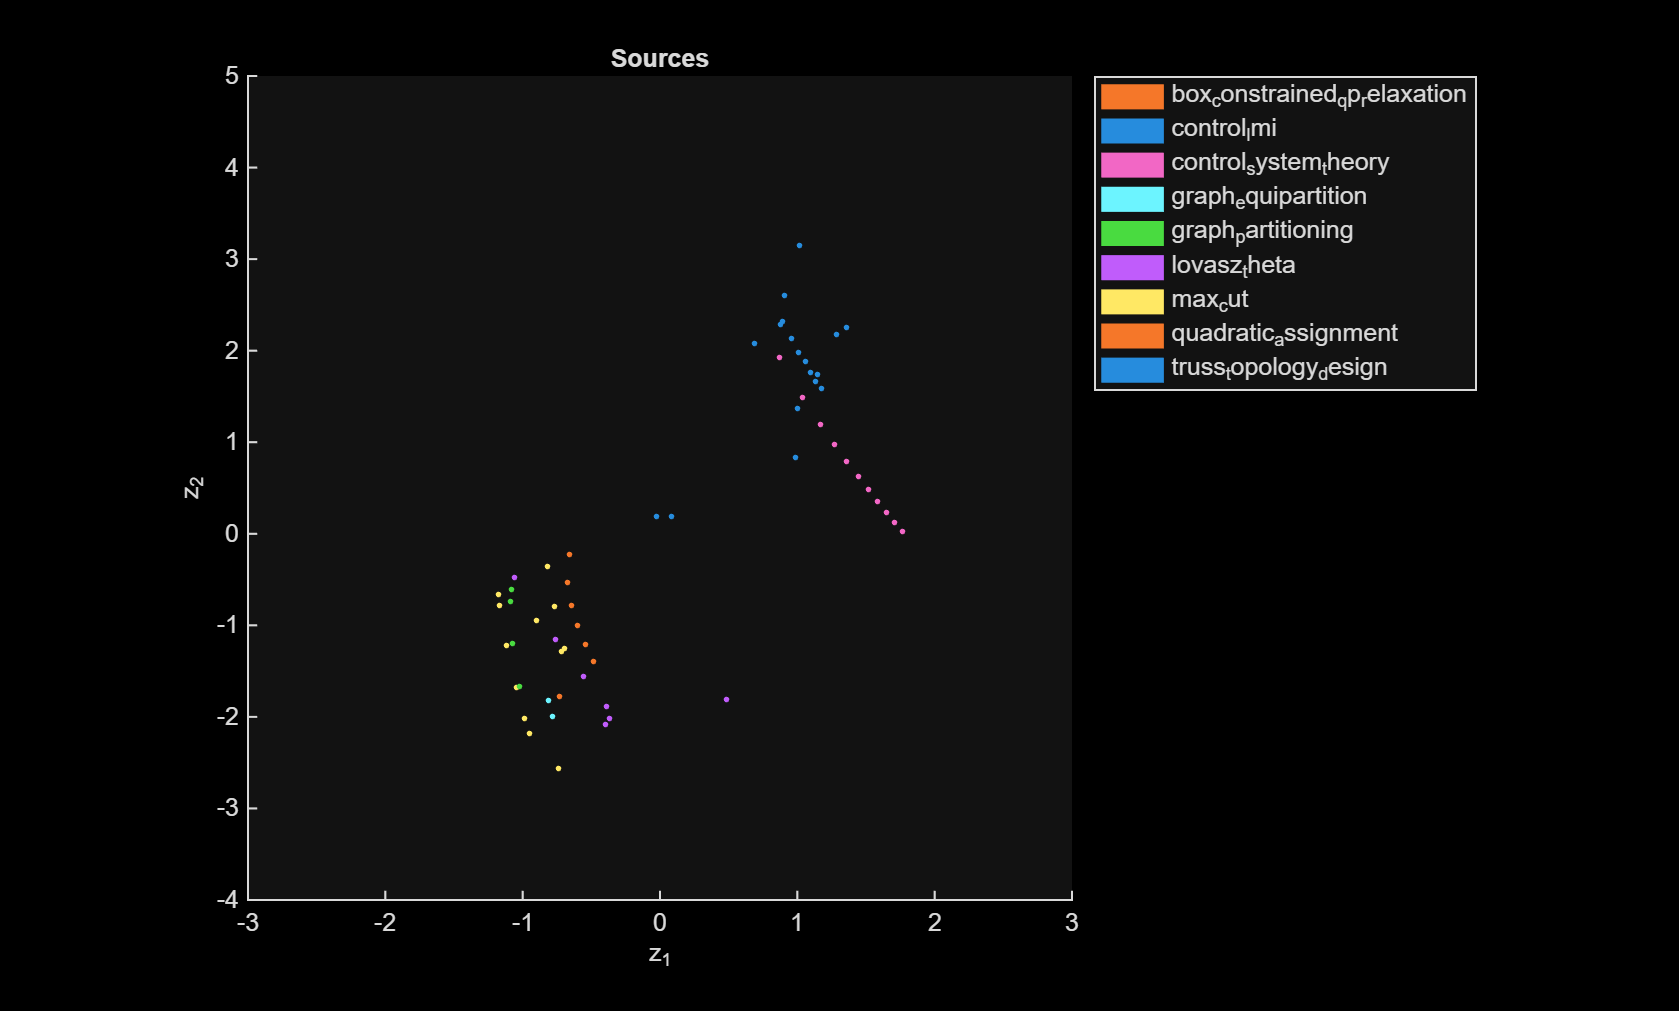
\includegraphics[width=0.82\textwidth]{isa_distribution_sources.png}
    \caption{Ejemplo de distribución de instancias en un espacio bidimensional, separadas por
    fuente o familia de origen.}
    \label{fig:isa_sources}
\end{figure}

\subsection{Construcción del espacio de instancias}
\label{subsec:isa_space_construction}

La construcción del espacio de instancias se organiza en una secuencia de etapas. La primera,
PRELIM (\textit{Preparation for Learning of Instance Meta-Data}), prepara los metadatos para el
aprendizaje posterior. En esta etapa se define, a partir de un umbral especificado por el usuario,
una medida binaria de buen desempeño para cada par algoritmo-instancia. Además, se aplican
procedimientos de acotamiento y normalización para reducir el efecto de valores extremos y hacer
comparables las escalas de las distintas características y métricas de rendimiento.

La segunda etapa, SIFTED (\textit{Selection of Instance Features to Explain Difficulty}), selecciona
un subconjunto de características informativas. La selección busca conservar variables que estén
correlacionadas con el desempeño de los algoritmos y, al mismo tiempo, eliminar redundancias
entre características similares. De esta forma, el espacio proyectado se construye con features que
aportan información sobre la dificultad de las instancias y sobre las diferencias de comportamiento
entre algoritmos.

La tercera etapa, PILOT (\textit{Projecting Instances with Linearly Observable Trends}), construye
la proyección bidimensional. A diferencia de técnicas generales de reducción de dimensionalidad,
como PCA, PILOT no busca únicamente preservar varianza. Su objetivo es encontrar una
transformación lineal que haga observables tendencias entre las coordenadas del espacio, las
características seleccionadas y las métricas de rendimiento. En términos generales, si
$\tilde f_j$ denota el vector de características seleccionado y normalizado para la instancia $x_j$,
la proyección puede entenderse como
\[
    z_j = P\tilde f_j,
\]
donde $P$ es una matriz de proyección aprendida desde los metadatos. Esta construcción permite
interpretar los ejes del espacio como combinaciones lineales de las características más relevantes.

La cuarta etapa, CLOISTER (\textit{Correlated Limits of the Instance Space's Theoretical or
Experimental Regions}), estima la frontera del espacio de instancias. Esta frontera no se limita al
convex hull de las instancias observadas, sino que intenta aproximar la región factible inducida por
los límites superiores e inferiores de las características, considerando también correlaciones entre
ellas. La frontera cumple un rol metodológico importante: permite evaluar si el conjunto de
instancias disponible cubre de forma diversa el espacio posible o si se concentra en una región
estrecha, dejando zonas sin evidencia experimental.

Una vez construido el espacio, la metodología incorpora modelos predictivos para selección
automática de algoritmos. En particular, PYTHIA entrena clasificadores SVM sobre las coordenadas
bidimensionales para predecir si un algoritmo tendrá buen desempeño en una instancia dada. Así,
una nueva instancia puede ser caracterizada mediante sus features, proyectada al espacio
bidimensional y asociada al algoritmo con mayor probabilidad de buen rendimiento.

El análisis de fortalezas y debilidades se realiza mediante footprints de algoritmos. Un footprint
corresponde a la región del espacio donde existe evidencia de que un algoritmo presenta buen
desempeño o desempeño superior respecto de los demás. Smith-Miles y Muñoz proponen TRACE
(\textit{Triangulation with Removal of Areas with Contradicting Evidence}) para construir estas
regiones y cuantificarlas mediante métricas como área, densidad y pureza. El área aproxima la
robustez del algoritmo en el espacio estudiado; la densidad indica cuánta evidencia empírica
sustenta la región; y la pureza mide si existen o no observaciones contradictorias dentro del
footprint.

La Figura~\ref{fig:isa_footprint_csdp} ilustra esta idea para un algoritmo particular: las zonas
marcadas como GOOD representan regiones del espacio donde el algoritmo cumple el criterio de
buen desempeño, mientras que las zonas BAD muestran instancias donde dicho criterio no se
alcanza. La forma y extensión de estas regiones permiten interpretar visualmente la cobertura y
robustez del algoritmo.

\begin{figure}[H]
    \centering
    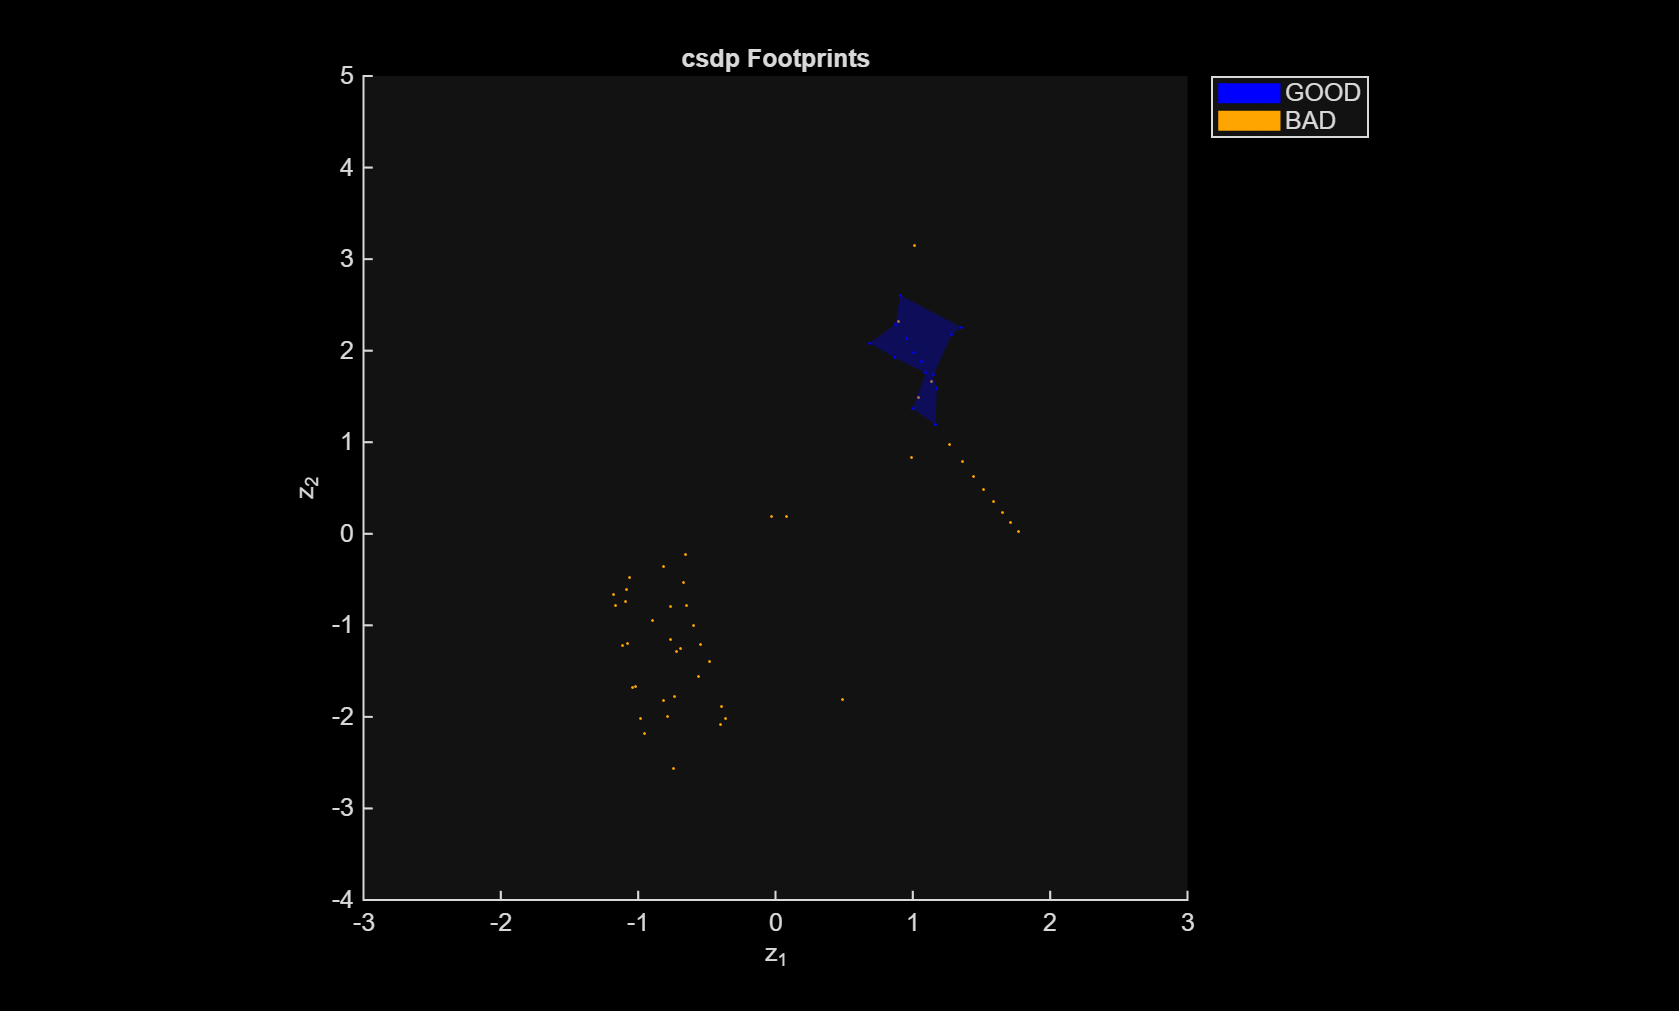
\includegraphics[width=0.82\textwidth]{isa_footprint_csdp.png}
    \caption{Ejemplo de footprint de desempeño para un algoritmo en el espacio de instancias.}
    \label{fig:isa_footprint_csdp}
\end{figure}

La metodología completa es iterativa. Un primer análisis puede revelar que las instancias
disponibles no son suficientemente diversas, que las características no explican adecuadamente el
rendimiento, o que el portafolio de algoritmos no permite observar diferencias claras. En esos
casos, \acrshort{isa} recomienda enriquecer los metadatos mediante nuevas instancias, nuevas
características o nuevos algoritmos, y repetir el proceso. Esta naturaleza iterativa convierte a
\acrshort{isa} no solo en una técnica de visualización, sino en una herramienta para diseñar
benchmarks más informativos y para realizar pruebas de algoritmos más objetivas y
estructuradas~\cite{smith-milesInstanceSpaceAnalysis2023}.
